
\subsection{Database Elasticsearch}\label{sec:db}

% introduction, users
\databaseName{} is a widely used non-relational database, which was designed to store and perform full-text search on a large corpus of unstructured data \cite{Elasticsearch2017}.
This open-source distributed document-driven database system is built in Java and is based on the Apache Lucene (Java) library for high-speed full-text search \cite{Elasticsearch2017, Elasticsearch2019}.
According to \citeauthor{Elasticsearch2019}, \databaseName{} provides Wikipedia's full-text search and suggestions as well as Github's code search and Stack Overflow's geolocation queries and related questions.
It enables near real-time search by index refreshing periods of one second.
Needless to say, \databaseName{} is qualified to handle Big Data.

% structure
\databaseName{} is a document store, which stores schemaless key-value pairs called documents \cite{flask2018}.
The documents are stored in logical units, so-called indices.
% index
As stated by \citeauthor{Elasticsearch2019} and \citeauthor{Elasticsearch2017}, the indices are structured similarly to Apache Lucene's inverted index format.
An index can be spread into multiple nodes.
A node is a single running instance of \databaseName{} \cite{Elasticsearch2019}.
An index is divided into one or more shards, which can be stored on different servers and enable parallelization.
% Replicas
Replicas are copies of shards, which create redundancy and thus, ensure availability. %\cite{Elasticsearch2019}.

% document
The documents are saved in a \ac{json} format \cite{Elasticsearch2017}.
A document's fields and field types are defined by the user when initializing the database index.
By default, every field of a document is indexed and searchable \cite{Elasticsearch2019}.

% query (endpoints)
% get: search id
By specifying the unique \texttt{\_id} of a document and the database \texttt{index}, it is possible to retrieve a specific document from the database using the \texttt{GET \ac{api}}.
The query is real-time by default.
The parameters \texttt{\_source\_excludes} or \texttt{\_source\_includes} can be used to define the structure of the response \cite{Elasticsearch-get}.

% full-text search
The keyword used when performing a full-text search is \texttt{match}.
To query for a specific value, one has to specify the \texttt{<field>} of interest and the query value.

\databaseName{} preprocesses the query value before starting the search \cite{Elasticsearch-text-analyser}.
The default preprocessing steps of the so-called default analyzer include tokenization and lowercasing \cite{Elasticsearch-text-analyser}. 
Omitting stop words is disabled by default, but it is possible to provide custom stop words or use the English stop word list \cite{Elasticsearch-text-analyser}.
It is possible to create custom tokenizers, which split the query value into tokens of a certain maximum length.

Another useful feature of \databaseName{} is the multi-term synonym expansion.
When the user queries a specific phrase \databaseName{} expands the query to include synonyms of the query terms \cite{Elasticsearch-synonyms}.
The maximum number of expansion terms is set to 50 by default but can be configured by the user \cite{Elasticsearch-match}.
By default, the multi-terms synonym expansion option is enabled.

\databaseName{} also provides the option to perform fuzzy matching instead of exact search.
By enabling the fuzzy matching option, a \databaseName{} query consisting of for instance, \textit{Bahama} returns documents that contain the word \textit{Bahamas}.
By default, this option is not enabled but can be enabled and configured individually by the user \cite{Elasticsearch-match}.


% knn-search
Another search option of \databaseName{} is the \ac{knn} search.
The return value of a \ac{knn} search is the \texttt{k} nearest neighbours in terms of a certain distance function of a query vector \cite{Elasticsearch-kNN-HNSW}.
The query is a dense vector of the same dimension as the vectors stored in the database.
A \ac{knn} search either returns the exact brute-force nearest neighbours or 
an approximation of the nearest neighbours calculated by the \ac{hnsw} algorithm \cite{Elasticsearch-kNN-HNSW, Elasticsearch-knn}.
\ac{hnsw} is a graph-based algorithm \cite{Elasticsearch-kNN-HNSW}.
The term \texttt{navigable} refers to the graphs used, which are graphs with (poly-)logarithmic scaling of links traversed during greedy traversal concerning the network size \cite{Elasticsearch-kNN-HNSW}.
The idea of a \texttt{hiercharical} algorithm is to create a multilayer graph, grouping links according to their link length, as displayed in \autoref{fig:hnsw-layer}. 
The search starts on the uppermost layer, i.e. the layer containing the longest links, greedily traversing the layer until reaching the local minimum.
It uses this local minimum as the starting point at the next lower layer and the process is repeated until the lowest layer is reached \cite{Elasticsearch-kNN-HNSW}.
The layers of the graph are built incrementally, and a neighbour selection heuristic, as depicted in \autoref{fig:hnsw-heuristic}, not only creates links between close elements, 
but also between isolated clusters to ensure global connectivity \cite{Elasticsearch-kNN-HNSW}.

\begin{figure}[!htb] % htp = hier (h), top (t), oder auf einer eigenen Seite (p).
    \centering
    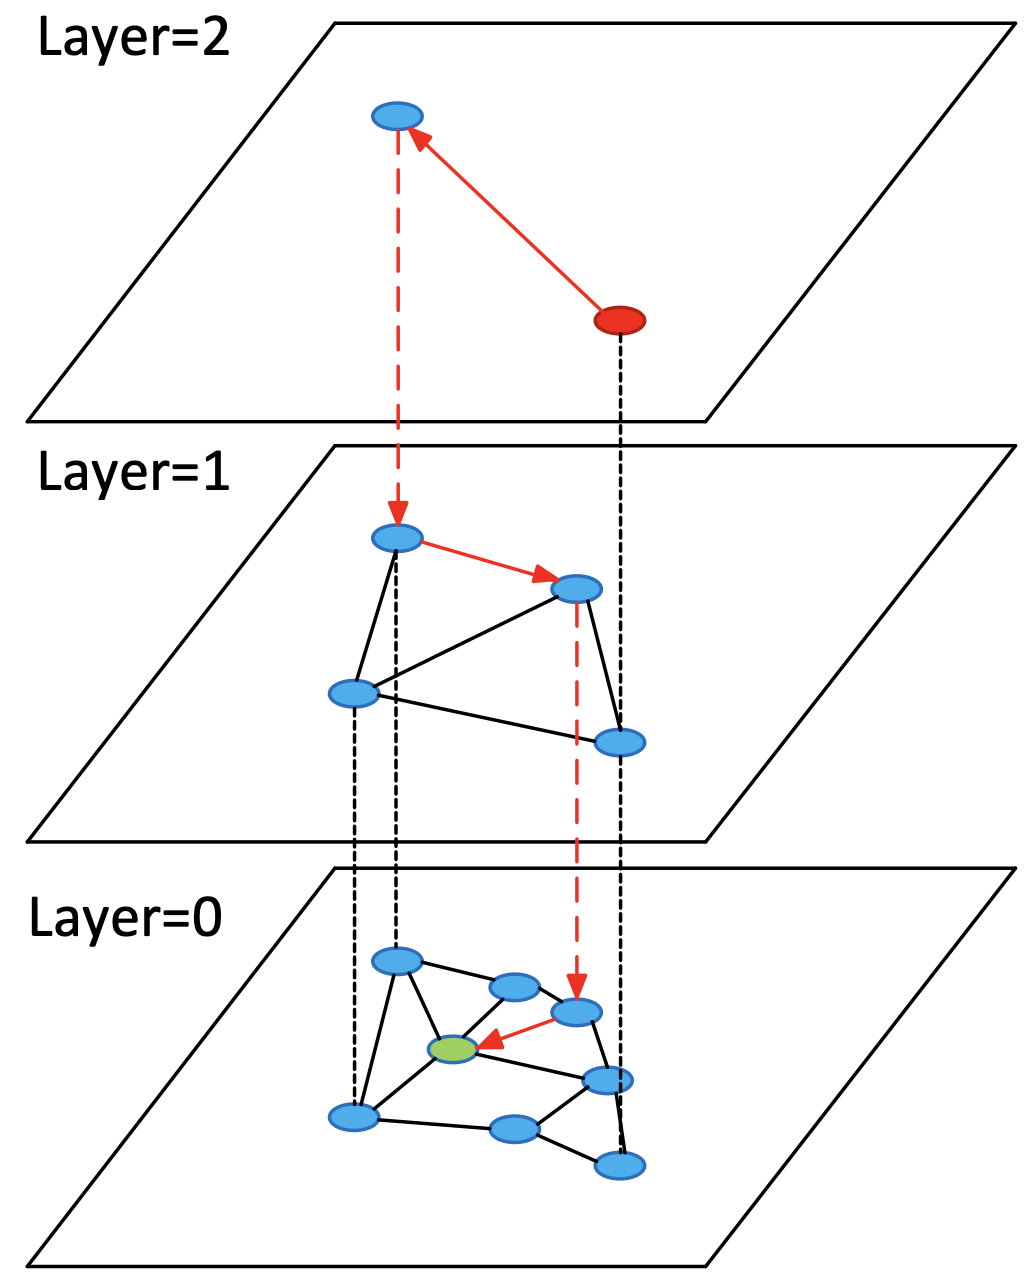
\includegraphics[width=0.4\textwidth]{images/Elasticsearch/HNSW-layer.png}
    \caption[Structure of \ac{hnsw} layers]{Structure of \ac{hnsw} layers from \cite{Elasticsearch-kNN-HNSW}.
    The search starts on the uppermost layer, i.e. the layer containing the longest links, greedily traversing the layer until reaching the local minimum.
    The local minimum is used as the starting point at the next lower layer and the process is repeated until the lowest layer is reached.
    }
    \label{fig:hnsw-layer}
\end{figure}

\begin{figure}[!htb] % htp = hier (h), top (t), oder auf einer eigenen Seite (p).
    \centering
    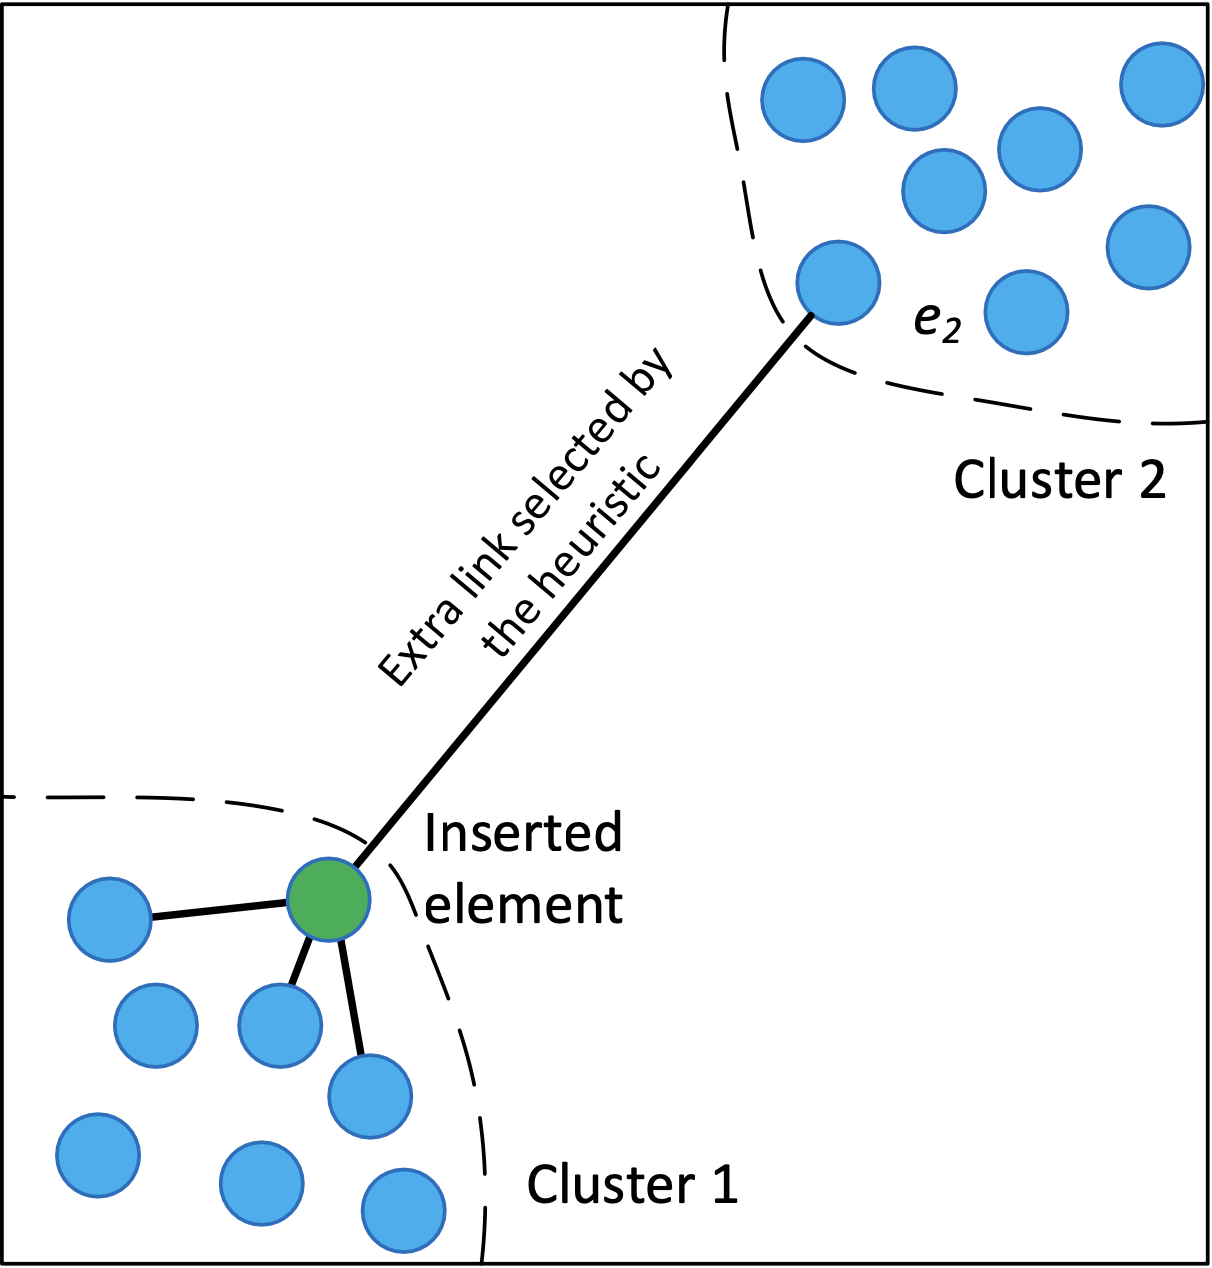
\includegraphics[width=0.5\textwidth]{images/Elasticsearch/HNSW-neighbour-selection-heuristic.png}
    \caption[Neighbour selection heuristic of \ac{hnsw}]{Neighbour selection heuristic of \ac{hnsw} from \cite{Elasticsearch-kNN-HNSW}.
    The heuristic creates diverse links, i.e. links between close elements (e.g., green circle and elements in cluster 1) 
    and between isolated clusters (e.g., green circle and $e_2$) to ensure global connectivity.
    }
    \label{fig:hnsw-heuristic}
\end{figure}

In order to perform \ac{knn} search on a \texttt{<field>} it has to be of type \texttt{dense\_vector}, indexed and a \texttt{similarity} measure has to be defined when initializing the database \cite{Elasticsearch-knn}.
\databaseName{}'s \ac{knn} implementation not only allows literal matching on search terms but also semantic search \cite{Elasticsearch-knn}.

Besides \databaseName{}, the elastic stack offers other tools, for instance, Kibana, which provides a user interface to manage different models.
After saving a model in Kibana, it is possible to create a text embedding ingest pipeline, which embeds new documents or reindexes existing documents \cite{Elasticsearch-knn-embedding}.
